\documentclass{hw}

\usepackage{minted}

\begin{document}
\begin{enumerate}
\item The following equation for the temperature $T=T(t)$ represents a spherical thermocouple with
convective conditions and includes radiation exchange with its surrounding walls
\[
c_{2}{dT\over\dt}=-(T-T_{\infty}+c_{1}(T^{4}-T^{4}_{sur})).
\]
In this equation, $c_{1}=1.27575\times10^{-10}K^{-3}$ and $c_{2}=0.991667s$. If it is assumed that
$T_{\infty}=473.15$, $T_{sur}=673.15K$, and $T(0)=298.15K$, determine the time $t_{s}$ at which
$T(t_{s})=490.85K$.
\begin{quote}
We can start by expressing our derivative in a discreet form. This gives the equation
\[
c_{2}\left({T(n+1)-T(n)\over\Delta t}\right)=-(T-T_{\infty}+c_{1}(T^{4}-T^{4}_{sur})).
\]
Solving this for $T(n+1)$ gives
\[
T(n+1)=-{\Delta t\over c_{2}}(T-T_{\infty}+c_{1}(T^{4}-T^{4}_{sur})) + T.
\]
\end{quote}
We can model this simply in C:

\begin{minted}[fontsize=\footnotesize,linenos]{c}
#include <stdio.h>
#include <stdlib.h>
#include <math.h>
#include <unistd.h>

int main(int argc, const char* argv[]){
    float temps [10000];
    temps[0] = 298.15;
    float starttime = 0;
    float deltat;
    if(argc > 1)
        deltat = atof(argv[1]);
    else
        deltat = 0.001;
    float c2 = 0.991667;
    float c1 = 1.27575 * powf(10,-10);
    float tinf = 473.15;
    float tsur = powf(673.15,4);
    FILE* fp = fopen("data.txt","w+");
    int i = 0;
    for(i = 0; i < 10000 && temps[i] < 490.85; i++){
        if(i % 10 == 0){
            fprintf(fp, "%f\n", temps[i]);
        }
        temps[i + 1] = (-1) * (deltat/c2) * (temps[i] - tinf + c1 * (pow(temps[i],4) - tsur)) + temps[i];
        starttime += deltat;
    }
    fclose(fp);
}
\end{minted}
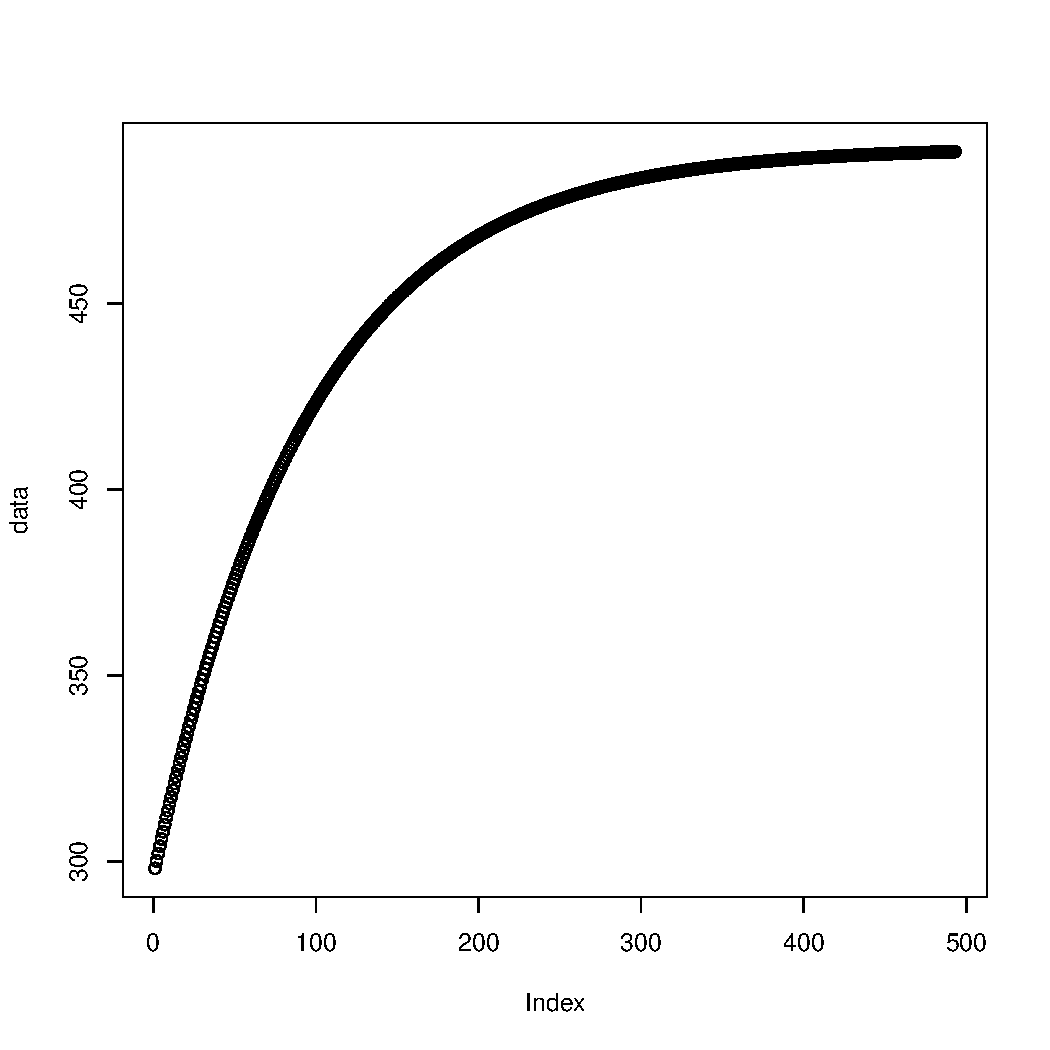
\includegraphics[scale=0.3]{Rplots}


\end{enumerate}
\end{document}
